\documentclass[12pt,oneside,a4paper]{book}

%\usepackage[utf8]{inputenc}
%\usepackage[T1]{fontenc}
\usepackage[english]{babel}

\usepackage{amsmath}
\usepackage{amssymb}
\usepackage{amsthm}
\usepackage{graphics}
\usepackage{amscd}
\usepackage{tikz}
\usetikzlibrary{shapes}

%%%% Layout %%%%%%%%%%%%%%%%%
\addtolength{\evensidemargin}{-2cm}
\addtolength{\oddsidemargin}{-2cm}
\setlength{\textwidth}{17cm} 
\setlength{\textheight}{26.5cm} 
\addtolength{\topmargin}{-3cm}
\setlength{\parindent}{0pt}
\pagestyle{plain}

\newcounter{probnum}
\newcounter{solnum}
\setcounter{probnum}{0}
\newcommand{\prob}{\ifnum\value{probnum}>0\newpage\fi\setcounter{solnum}{0}\stepcounter{probnum}\textbf{Problem \theprobnum}\\}
\newcommand{\ans}{\medskip\hrule\medbreak\emph{Answer: }}
\newcommand{\comment}{\medskip\hrule\medbreak\emph{Comment: }}
\newcommand{\sol}{\medskip\hrule\medbreak\textbf{Solution}\\}
\newcommand{\soln}{\stepcounter{solnum}\medskip\hrule\medbreak\textbf{Solution \thesolnum}\\}
\newcommand{\marking}{\medskip\hrule\medbreak\textbf{Marking scheme -- Problem \theprobnum}}

\newcommand*\circled[1]{\tikz[baseline=(char.base)]{
            \node[shape=circle,draw,inner sep=2pt] (char) {#1};}}

\newcommand{\s}{\phantom{s}}

\begin{document}
\begin{center}
\textbf{\large APMO 2004 -- Problems and Solutions}
\end{center}

% Problem 1
\prob Determine all finite nonempty sets $S$ of positive integers satisfying
\[\frac{i+j}{(i,j)}\quad\text{is an element of }S\text{ for all }i,j\text{ in }S,\]
where $(i,j)$ is the greatest common divisor of $i$ and $j$.

\ans $S = \{2\}$.

\sol
Let $k\in S$. Then $\frac{k+k}{(k,k)} = 2$ is in $S$ as well.

Suppose for the sake of contradiction that there is an odd number in $S$, and let $k$ be the largest such odd number. Since $(k,2)=1$, $\frac{k+2}{(k,2)} = k+2 > k$ is in $S$ as well, a contradiction. Hence $S$ has no odd numbers.

Now suppose that $\ell > 2$ is the second smallest number in $S$. Then $\ell$ is even and $\frac{\ell+2}{(\ell,2)} = \frac\ell2 + 1$ is in $S$. Since $\ell > 2 \implies \frac\ell2 + 1 > 2$, $\frac\ell2 + 1 \ge \ell\iff\ell \le 2$, a contradiction again.

Therefore $S$ can only contain $2$, and $S=\{2\}$ is the only solution.

% Problem 2
\prob Let $O$ be the circumcentre and $H$ the orthocentre of an acute triangle $ABC$. Prove that the area of one of the triangles $AOH$, $BOH$ and $COH$ is equal to the sum of the areas of the other two.

\soln
Suppose, without loss of generality, that $B$ and $C$ lies in the same side of line $OH$. Such line is the \emph{Euler line} of $ABC$, so the centroid $G$ lies in this line.
\begin{center}
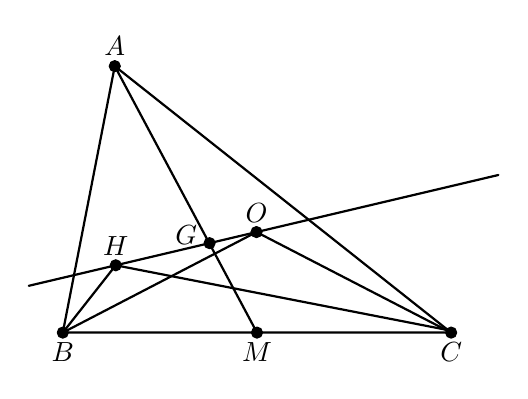
\begin{tikzpicture}[line cap=round,line join=round,x=0.6cm,y=0.6cm]
\draw [thick] (2.26,2.08) node[anchor=south] {$A$} -- (1.16,-3.56) node[anchor=north] {$B$} -- (9.38,-3.56) node[anchor=north] {$C$} -- cycle;
\draw [thick, domain=0.44:10.38] plot(\x,{(-7.964946939339505--0.7030223158767446*\x)/2.979231034959237});
\draw [thick] (1.16,-3.56)-- (2.2805126433605087,-2.1353482105844965);
\draw [thick] (1.16,-3.56)-- (5.2597436783197455,-1.432325894707752);
\draw [thick] (5.2597436783197455,-1.432325894707752)-- (9.38,-3.56);
\draw [thick] (9.38,-3.52)-- (2.2805126433605087,-2.1353482105844965);
\draw [thick] (2.26,2.08)-- (5.27,-3.56);
\draw [fill=black] (2.26,2.08) circle (2pt);
\draw [fill=black] (1.16,-3.56) circle (2pt);
\draw [fill=black] (9.38,-3.56) circle (2pt);
\draw [fill=black] (2.2805126433605087,-2.1353482105844965) circle (2.0pt) node[anchor=south] {$H$};
\draw [fill=black] (5.2597436783197455,-1.432325894707752) circle (2.0pt) node[anchor=south] {$O$};
\draw [fill=black] (4.266666666666667,-1.6666666666666667) circle (2.0pt) node[above=3pt, left=1pt] {$G$};
\draw [fill=black] (5.27,-3.56) circle (2.0pt) node[anchor=north] {$M$};
\end{tikzpicture}
\end{center}

Let $M$ be the midpoint of $BC$. Then the distance between $M$ and the line $OH$ is the average of the distances from $B$ and $C$ to $OH$, and the sum of the areas of triangles $BOH$ and $COH$ is
\[[BOH] + [COH] = \frac{OH\cdot d(B,OH)}2 + \frac{OH\cdot d(C,OH)}2 = \frac{OH\cdot 2d(M,OH)}2.\]

Since $AG = 2GM$, $d(A,OH) = 2d(M,OH)$. Hence
\[[BOH] + [COH] = \frac{OH\cdot d(A,OH)}2 = [AOH],\]
and the result follows.

\soln
One can use barycentric coordinates: it is well known that
\[\displaylines{A = (1:0:0), \quad B=(0:1:0), \quad C=(0:0:1),\cr
O = (\sin 2A : \sin 2B : \sin 2C)\quad\text{and}\quad H = (\tan A : \tan B : \tan C).}\]

Then the (signed) area of $AOH$ is proportional to
\[\left|\begin{matrix}
1& 0& 0\\
\sin 2A& \sin 2B& \sin 2C\\
\tan A& \tan B& \tan C
\end{matrix}\right|
\]

Adding all three expressions we find that the sum of the signed sums of the areas is a constant times
\[\left|\begin{matrix}
1& 0& 0\\
\sin 2A& \sin 2B& \sin 2C\\
\tan A& \tan B& \tan C
\end{matrix}\right|
+
\left|\begin{matrix}
0& 1& 0\\
\sin 2A& \sin 2B& \sin 2C\\
\tan A& \tan B& \tan C
\end{matrix}\right|
+
\left|\begin{matrix}
0& 0& 1\\
\sin 2A& \sin 2B& \sin 2C\\
\tan A& \tan B& \tan C
\end{matrix}\right|.\]

By multilinearity of the determinant, this sum equals
\[\left|\begin{matrix}
1& 1& 1\\
\sin 2A& \sin 2B& \sin 2C\\
\tan A& \tan B& \tan C
\end{matrix}\right|,
\]
which contains, in its rows, the coordinates of the centroid, the circumcenter, and the orthocenter. Since these three points lie in the Euler line of $ABC$, the signed sum of the areas is $0$, which means that one of the areas of $AOH,BOH,COH$ is the sum of the other two areas.

\comment
Both solutions can be adapted to prove a stronger result: if the centroid $G$ of triangle $ABC$ belongs to line $XY$ then one of the areas of triangles $AXY$, $BXY$, and $CXY$ is equal to the sum of the other two.

% Problem 3
\prob Let a set $S$ of $2004$ points in the plane be given, no three of which are collinear. Let $\mathcal{L}$ denote the set of all lines (extended indefinitely in both directions) determined by pairs of points from the set. Show that it is possible to colour the points of $S$ with at most two colours, such that for any points $p,q$ of $S$, the number of lines in $\mathcal{L}$ which separate $p$ from $q$ is odd if and only if $p$ and $q$ have the same colour.

\emph{Note}: A line $\ell$ separates two points $p$ and $q$ if $p$ and $q$ lie on opposite sides of $\ell$ with neither point on $\ell$.

\sol Choose any point $p$ from $S$ and color it, say, blue. Let $n(q,r)$ be the number of lines from $\mathcal{L}$ that separates $q$ and $r$. Then color any other point $q$ blue if $n(p,q)$ is odd and red if $n(p,q)$ is even.

Now it remains to show that $q$ and $r$ have the same color if and only if $n(q,r)$ is odd for all $q\ne p$ and $r\ne p$, which is equivalent to proving that $n(p,q) + n(p,r) + n(q,r)$ is always odd. For this purpose, consider the seven numbered regions defined by lines $pq$, $pr$, and $qr$:
\begin{center}
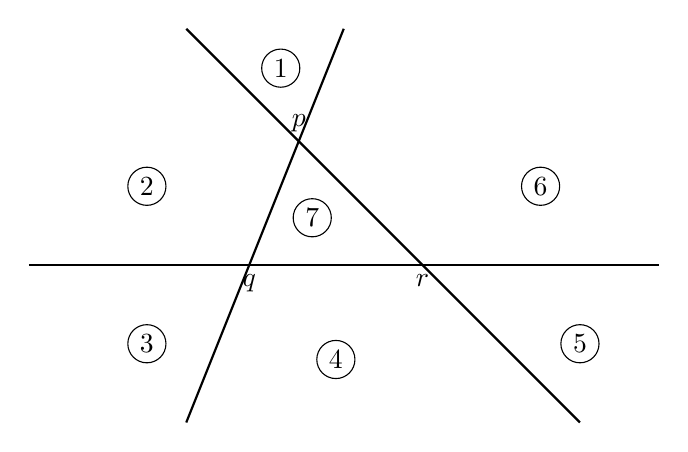
\begin{tikzpicture}
\draw[thick] (-4,0) -- (4,0);
\draw[thick] (-2,-2) -- (0,3);
\draw[thick] (-2,3) -- (3,-2);
\draw (-0.57,1.57) node[anchor=south] {$p$};
\draw (-1.2,0) node[anchor=north] {$q$};
\draw (1,0) node[anchor=north] {$r$};
\draw (-0.8,2.5) node {\circled{1}};
\draw (-2.5,1) node {\circled{2}};
\draw (-2.5,-1) node {\circled{3}};
\draw (-0.1,-1.2) node {\circled{4}};
\draw (3,-1) node {\circled{5}};
\draw (2.5,1) node {\circled{6}};
\draw (-0.4,0.6) node {\circled{7}};
\end{tikzpicture}
\end{center} 

Any line that do not pass through any of points $p,q,r$ meets the sides $pq,qr,pr$ of triangle $pqr$ in an even number of points (two sides or no sides), so these lines do not affect the parity of $n(p,q) + n(p,r) + n(q,r)$. Hence the only lines that need to be considered are the ones that pass through one of vertices $p,q,r$ and cuts the opposite side in the triangle $pqr$.

Let $n_i$ be the number of points in region $i$, $p$, $q$, and $r$ excluded, as depicted in the diagram. Then the lines through $p$ that separate $q$ and $r$ are the lines passing through $p$ and points from regions $1$, $4$, and $7$. The same applies for $p,q$ and regions $2$, $5$, and $7$; and $p,r$ and regions $3$, $6$, and $7$. Therefore
\begin{align*}
n(p,q) + n(q,r) + n(p,r) &\equiv (n_2 + n_5 + n_7) + (n_1 + n_4 + n_7) + (n_3 + n_6 + n_7) \\
&\equiv n_1 + n_2 + n_3 + n_4 + n_5 + n_6 + n_7 = 2004 - 3 \equiv 1 \pmod 2,
\end{align*}
and the result follows.

\comment The problem statement is also true if $2004$ is replaced by any even number and is not true if $2004$ is replaced by any odd number greater than $1$.

% Problem 4
\prob For a real number $x$, let $\lfloor x\rfloor$ stand for the largest integer that is less than or equal to $x$. Prove that
\[\left\lfloor\frac{(n-1)!}{n(n+1)}\right\rfloor\]
is even for every positive integer $n$.

\sol
Consider four cases:
\begin{itemize}
\item $n\le 5$. Then $\left\lfloor\frac{(n-1)!}{n(n+1)}\right\rfloor = 0$ is an even number.
\item \emph{$n$ and $n+1$ are both composite (in particular, $n\ge 8$)}. Then $n=ab$ and $n+1=cd$ for $a,b,c,d\ge 2$. Moreover, since $n$ and $n+1$ are coprime, $a,b,c,d$ are all distinct and smaller than $n$, and one can choose $a,b,c,d$ such that exactly one of these four numbers is even. Hence $\frac{(n-1)!}{n(n+1)}$ is an integer. As $n\ge 8 > 6$, $(n-1)!$ has at least three even factors, so $\frac{(n-1)!}{n(n+1)}$ is an even integer.
\item \emph{$n\ge 7$ is an odd prime}. By Wilson's theorem, $(n-1)!\equiv-1\pmod n$, that is, $\frac{(n-1)!+1}n$ is an integer, as $\frac{(n-1)!+n+1}n = \frac{(n-1)!+1}n+1$ is. As before, $\frac{(n-1)!}{n+1}$ is an even integer; therefore $\frac{(n-1)! + n+1}{n+1} = \frac{(n-1)!}{n+1} + 1$ is an odd integer.

Also, $n$ and $n+1$ are coprime and $n$ divides the odd integer $\frac{(n-1)! + n+1}{n+1}$, so $\frac{(n-1)!+n+1}{n(n+1)}$ is also an odd integer. Then
\[\left\lfloor\frac{(n-1)!}{n(n+1)}\right\rfloor = \frac{(n-1)!+n+1}{n(n+1)} - 1\]
is even.
\item \emph{$n+1\ge 7$ is an odd prime}. Again, since $n$ is composite, $\frac{(n-1)!}n$ is an even integer, and $\frac{(n-1)!+n}n$ is an odd integer. By Wilson's theorem, $n!\equiv -1\pmod{n+1}\iff (n-1)!\equiv 1\pmod{n+1}$. This means that $n+1$ divides $(n-1)! + n$, and since $n$ and $n+1$ are coprime, $n+1$ also divides $\frac{(n-1)!+n}n$. Then $\frac{(n-1)!+n}{n(n+1)}$ is also an odd integer and
\[\left\lfloor\frac{(n-1)!}{n(n+1)}\right\rfloor = \frac{(n-1)!+n}{n(n+1)} - 1\]
is even.
\end{itemize}

% Problem 5
\prob Prove that
\[(a^2+2)(b^2+2)(c^2+2) \ge 9(ab+bc+ca)\]
for all real numbers $a,b,c>0$.

\soln
Let $p=a+b+c$, $q=ab+bc+ca$, and $r=abc$. The inequality simplifies to
\[a^2b^2c^2 + 2(a^2b^2 + b^2c^2 + c^2a^2) + 4(a^2+b^2+c^2) + 8 - 9(ab+bc+ca) \ge 0.\]

Since $a^2b^2+b^2c^2+c^2a^2 = q^2 - 2pr$ and $a^2+b^2+c^2 = p^2-2q$,
\[r^2 + 2q^2 - 4pr + 4p^2 - 8q + 8 - 9q \ge 0,\]
which simplifies to
\[r^2 + 2q^2 + 4p^2 - 17q - 4pr + 8\ge 0.\eqno{(I)}\]

Bearing in mind that equality occurs for $a=b=c=1$, which means that, for instance, $p=3r$, one can rewrite $(I)$ as
\[\left(r-\frac p3\right)^2 - \frac{10}3pr + \frac{35}9p^2 + 2q^2 - 17q + 8 \ge 0.\eqno{(II)}\]

Since $(ab-bc)^2 + (bc-ca)^2 + (ca-ab)^2 \ge 0$ is equivalent to $q^2 \ge 3pr$, rewrite $(II)$ as
\[\left(r-\frac p3\right)^2 + \frac{10}9(q^2-3pr) + \frac{35}9p^2 + \frac89q^2 - 17q + 8 \ge 0.\eqno{(III)}\]

Finally, $a=b=c=1$ implies $q=3$; then rewrite $(III)$ as
\[\left(r-\frac p3\right)^2 + \frac{10}9(q^2-3pr) + \frac{35}9(p^2-3q) + \frac89(q-3)^2 \ge 0.\]

This final inequality is true because $q^2\ge 3pr$ and $p^2 - 3q = \frac12[(a-b)^2 + (b-c)^2 + (c-a)^2] \ge 0$.

\soln
We prove the stronger inequality
\[(a^2+2)(b^2+2)(c^2+2) \ge 3(a+b+c)^2,\eqno{(*)}\]
which implies the proposed inequality because $(a+b+c)^2 \ge 3(ab+bc+ca)$ is equivalent to $(a-b)^2 + (b-c)^2 + (c-a)^2\ge 0$, which is immediate.

The inequality $(*)$ is equivalent to
\[\bigl((b^2+2)(c^2+2)-3\bigr)a^2 - 6(b+c)a + 2(b^2+2)(c^2+2) - 3(b+c)^2 \ge 0.\]

Seeing this inequality as a quadratic inequality in $a$ with positive leading coefficient $(b^2+2)(c^2+2)-3 = b^2c^2 + 2b^2 + 2c^2 + 1$, it suffices to prove that its discriminant is non-positive, which is equivalent to
\[(3(b+c))^2 - \bigl((b^2+2)(c^2+2)-3\bigr)\bigl(2(b^2+2)(c^2+2) - 3(b+c)^2\bigr) \le 0.\]

This simplifies to
\[-2(b^2+2)(c^2+2) + 3(b+c)^2 + 6 \le 0.\eqno{(**)}\]

Now we look $(**)$ as a quadratic inequality in $b$ with negative leading coefficient $-2c^2-1$:
\[(-2c^2-1)b^2 + 6cb - c^2-2\le 0.\]

If suffices to show that the discriminant of $(**)$ is non-positive, which is equivalent to
\[9c^2 - (2c^2+1)(c^2+2) \le 0.\]

It simplifies to $-2(c^2-1)^2 \le 0$, which is true. The equality occurs for $c^2=1$, that is, $c=1$, for which $b = \frac{6c}{2(2c^2+1)} = 1$, and $a = \frac{6(b+c)}{2((b^2+2)(c^2+2)-3)} = 1$.

\soln
Let $A,B,C$ angles in $(0,\pi/2)$ such that $a = \sqrt 2\tan A$, $b = \sqrt 2\tan B$, and $c = \sqrt 2\tan C$. Then the inequality is equivalent to
\[4\sec^2A\sec^2B\sec^2C \ge 9(\tan A\tan B + \tan B\tan C + \tan C\tan A).\]

Substituting $\sec x = \frac1{\cos x}$ for $x\in\{A,B,C\}$ and clearing denominators, the inequality is equivalent to
\[\cos A\cos B\cos C(\sin A\sin B\cos C + \cos A\sin B\sin C + \sin A\cos B\sin C) \le \frac49.\]

Since
\begin{align*}
&\cos(A+B+C) = \cos A\cos(B+C) - \sin A\sin(B+C)\\
{}={}& \cos A\cos B\cos C - \cos A\sin B\sin C - \sin A\cos B\sin C - \sin A\sin B\cos C,
\end{align*}
we rewrite our inequality as
\[\cos A\cos B\cos C(\cos A\cos B\cos C - \cos(A+B+C)) \le \frac49.\]

The cosine function is concave down on $(0,\pi/2)$. Therefore, if $\theta = \frac{A+B+C}3$, by the AM-GM inequality and Jensen's inequality,
\[\cos A\cos B\cos C \le \left(\frac{\cos A + \cos B + \cos C}3\right)^3 \le \cos^3\frac{A+B+C}3 = \cos^3\theta.\]

Therefore, since $\cos A\cos B\cos C - \cos(A+B+C) = \sin A\sin B\cos C + \cos A\sin B\sin C + \sin A\cos B\sin C > 0$, and recalling that $\cos3\theta = 4\cos^3\theta-3\cos\theta$,
\[\cos A\cos B\cos C(\cos A\cos B\cos C - \cos(A+B+C)) \le \cos^3\theta(\cos^3\theta - \cos3\theta)
= 3\cos^4\theta(1-\cos^2\theta).\]

Finally, by AM-GM (notice that $1-\cos^2\theta = \sin^2\theta > 0$),
\[3\cos^4\theta(1-\cos^2\theta) = \frac32\cos^2\theta\cdot \cos^2\theta(2-2\cos^2\theta) \le \frac32\left(\frac{\cos^2\theta + \cos^2\theta + (2-2\cos^2\theta)}3\right)^3 = \frac49,\]
and the result follows.

\end{document}